% !TEX encoding = UTF-8 Unicode
\documentclass[a4paper,12pt]{article}

%-----------------------------------------Include package & set up some thing-----------------------------------------------
\usepackage{fontspec}
\setmainfont{Times New Roman} %set font
\usepackage{enumitem} % to format list
\usepackage{amsmath}
\usepackage{listings} % quote code
\usepackage{color}
\usepackage{hyperref} % cite hyperlink & bookmarks
\usepackage{setspace} % space
\usepackage{graphicx} % insert image
\usepackage{subcaption} % Multiple images
\usepackage{float}
\usepackage[margin=1in, footskip = 0.25in]{geometry} % Change margin with geometry package

\hypersetup{unicode, colorlinks,linkcolor=black, urlcolor=cyan} % format hyperlink and bookmarks

%Define title
\title{Báo cáo bài tập 5}
\author{1612174 - Phùng Tiến Hào - \href{mailto:tienhaophung@gmail.com}{tienhaophung@gmail.com}}
\date{28/04/2019}

%Code formatting with the listing package
\definecolor{codegreen}{rgb}{0,0.6,0}
\definecolor{codegray}{rgb}{0.3,0.3,0.3}
\definecolor{codepurple}{rgb}{0.58,0,0.82}
\definecolor{backcolour}{rgb}{0.92,0.92,0.88}

\lstdefinestyle{mystyle}{
	backgroundcolor=\color{backcolour},   
	commentstyle=\color{codegreen},
	keywordstyle=\color{blue},
	numberstyle=\tiny\color{codegray},
	stringstyle=\color{codepurple},
	basicstyle=\footnotesize,
	breakatwhitespace=false,         
	breaklines=true,                 
	captionpos=b,                    
	keepspaces=true,                 
	numbers=left,                    
	numbersep=5pt,                  
	showspaces=false,                
	showstringspaces=false,
	showtabs=false,                  
	tabsize=2,
	columns=fullflexible,
	frame=single
}

\lstset{style=mystyle}

\begin{document}
	\pagenumbering{gobble}
	\maketitle
	\newpage
	
	\doublespacing
	\tableofcontents
	\singlespace
	
	\newpage
	\pagenumbering{arabic}
	
	\textbf{Dữ liệu khảo sát:} SpeedDating trong package Lock5withR\\
	
	Load package và thêm các thư viện cần thiết trước khi đi vào xử lý:
	\begin{lstlisting}[language=R]
	require(Lock5withR) # Load package
	library(Lock5withR)
	library(mosaic)
	head(SpeedDating)
	attach(SpeedDating) # Avoid dollar sign before each varibles name
	\end{lstlisting}
	\section{Khảo sát một biến}
	\subsection{Biến định tính (Categorical variable)}
	\subsubsection{DecisionMale (Yes/No)}
	Giả sử, ta cần khảo sát tỉ lệ nam phản hồi (Yes/No) cho quần thể (population) là toàn bộ học sinh nam của trường Columbia. Từ tổng thể, ta thu thập được một mẫu dữ liệu ngẫu nhiên (random sample) gồm 276 quan sát trong đó có 146 phản hồi "Yes" và 130 phản hồi "No". Dựa vào mẫu dữ liệu này, ta xây dựng khoảng tin cậy
	(confident interval) 95\% cho tỉ lệ phản hồi "Yes"/"No" của sinh viên nam trường.
	\begin{enumerate}[label=\alph*)]
		\item Xây dựng khoảng tin cậy cho tỉ lệ phản hồi "Yes" của nam\\
		
		Gọi $p$ là tỉ lệ nam phản hồi "Yes" trong trường, $\hat{p}$ là tỉ lệ nam phản hồi "Yes" trong mẫu dữ liệu. Ta có
		$$\hat{p} = \frac{146}{276} = 0.529$$
		\begin{lstlisting}[language=R]
			# Cac TK can tinh
			stat <- function(data){
				return (sum(data == 'Yes')/length(data)) # Ti le
			}
			
			# Bootstrap
			bootstrap <- function(B){
				return (replicate(B, stat(sample(data, length(data), replace = TRUE))))
			}
			
			# Lay du lieu
			data <- DecisionMale
			
			(alpha <- 1 - 0.95)
			boots_dist <- bootstrap(10000) # Tim phan phoi cua bootstrap
			(se <- sd(boots_dist)) # Tinh standard deviation
			(conf_boots <- quantile(boots_dist, c(alpha/2, 1 - alpha/2))) # Tim khoang tin cay cho p
			
			# Run
			> (alpha <- 1 - 0.95)
			[1] 0.05
			> boots_dist <- bootstrap(10000) # Tim phan phoi cua bootstrap
			> (se <- sd(boots_dist)) # Tinh standard deviation
			[1] 0.02973836
			> (conf_boots <- quantile(boots_dist, c(alpha/2, 1 - alpha/2))) # Tim khoang tin cay cho p
			2.5%     97.5% 
			0.4709239 0.5869565 
		\end{lstlisting}
		
		Vậy sai số chuẩn xấp xỉ bằng bootstrap là 0.02973836 và khoảng tin cậy 95\% cho $p$ dựa trên bootstrap là [0.4709239 0.5869565].
		
		\item Xây dựng khoảng tin cậy cho tỉ lệ phản hồi "No" của nam\\
		
		Gọi $p$ là tỉ lệ nam phản hồi "No" trong trường, $\hat{p}$ là tỉ lệ nam phản hồi "No" trong mẫu dữ liệu. Ta có
		$$\hat{p} = \frac{130}{276} = 0.471$$
		\begin{lstlisting}[language = R]
		# Cac TK can tinh
		stat <- function(data){
			return (mean(data == 'No'))
		}
		
		(alpha <- 1 - 0.95)
		boots_dist <- bootstrap(10000) # Tim phan phoi cua bootstrap
		(se <- sd(boots_dist)) # Tinh standard deviation
		(conf_boots <- quantile(boots_dist, c(alpha/2, 1 - alpha/2))) # Tim khoang tin cay cho p
		
		# Run
		> (alpha <- 1 - 0.95)
		[1] 0.05
		> boots_dist <- bootstrap(10000) # Tim phan phoi cua bootstrap
		> (se <- sd(boots_dist)) # Tinh standard deviation
		[1] 0.03024206
		> (conf_boots <- quantile(boots_dist, c(alpha/2, 1 - alpha/2))) # Tim khoang tin cay cho p
		2.5%     97.5% 
		0.4130435 0.5289855
		\end{lstlisting}
		
		Vậy sai số chuẩn xấp xỉ bằng bootstrap là 0.03024206 và khoảng tin cậy 95\% cho $p$ dựa trên bootstrap là [0.4130435, 0.5289855].
		
	\end{enumerate}
	\textbf{Nhận xét:}\\
	\begin{itemize}
	\item Khoảng tin cậy cho tỉ lệ khác biệt giữa phản hồi "Yes" và "No":
	$$[0.4709239 0.5869565] - [0.4130435, 0.5289855] = [0.0578804, 0.057971]$$
	\item Điều này, cho thấy $p_{Yes} \geq p_{No}$
	\end{itemize}
	\subsubsection{RaceF (Caucasian, Asian,..., Other)}
	Giả sử, ta cần khảo sát tỉ lệ dân tộc nữ (Caucasian, Asian,..., Other) cho quần thể (population) là toàn bộ học sinh nữ của trường Columbia. Từ tổng thể, ta thu thập được một mẫu dữ liệu ngẫu nhiên (random sample) gồm 276 quan sát trong đó có 4 rỗng, 70 Asians, 15 Blacks, 148 Caucasians, 23 Latino và 16 Others. Dựa vào mẫu dữ liệu này, ta xây dựng khoảng tin cậy (confident interval) 95\% cho tỉ lệ dân tộc của sinh viên nữ trường.
	\begin{enumerate}[label = \alph*)]
		\item Xây dựng khoảng tin cậy cho tỉ lệ nữ da trắng (Caucasian)\\
		
		Gọi $p$ là tỉ lệ nữ da trắng trong trường, $\hat{p}$ là tỉ lệ nữ da trắng trong mẫu dữ liệu. Ta có
		$$\hat{p} = \frac{148}{276} = 0.536$$
			\begin{lstlisting}[language=R]
			# Cac TK can tinh
			stat <- function(data){
				return (sum(data == 'Caucasian')/length(data)) # Ti le
			}
			
			# Bootstrap
			bootstrap <- function(B){
				return (replicate(B, stat(sample(data, length(data), replace = TRUE))))
			}
			
			# Lay du lieu
			data <- RaceF
			
			(alpha <- 1 - 0.95)
			boots_dist <- bootstrap(10000) # Tim phan phoi cua bootstrap
			(se <- sd(boots_dist)) # Tinh standard deviation
			(conf_boots <- quantile(boots_dist, c(alpha/2, 1 - alpha/2))) # Tim khoang tin cay cho p
			
			#Run
			> (alpha <- 1 - 0.95)
			[1] 0.05
			> boots_dist <- bootstrap(10000) # Tim phan phoi cua bootstrap
			> (se <- sd(boots_dist)) # Tinh standard deviation
			[1] 0.03044327
			> (conf_boots <- quantile(boots_dist, c(alpha/2, 1 - alpha/2))) # Tim khoang tin cay cho p
			2.5%     97.5% 
			0.4782609 0.5978261
			\end{lstlisting}
			Vậy sai số chuẩn xấp xỉ bằng bootstrap là 0.03044327 và khoảng tin cậy 95\% cho $p$ dựa trên bootstrap
			là [0.4782609, 0.5978261].
		\item Xây dựng khoảng tin cậy cho tỉ lệ nữ da châu Á (Asian)\\
		
		Gọi $p$ là tỉ lệ nữ châu Á trong trường, $\hat{p}$ là tỉ lệ nữ châu Á trong mẫu dữ liệu. Ta có
		$$\hat{p} = \frac{70}{276} = 0.254$$
			\begin{lstlisting}[language=R]
			# Cac TK can tinh
			stat <- function(data){
				return (sum(data == 'Caucasian')/length(data)) # Ti le
			}
			
			# Bootstrap
			bootstrap <- function(B){
				return (replicate(B, stat(sample(data, length(data), replace = TRUE))))
			}
			
			# Lay du lieu
			data <- RaceF
			
			> (alpha <- 1 - 0.95)
			[1] 0.05
			> boots_dist <- bootstrap(10000) # Tim phan phoi cua bootstrap
			> (se <- sd(boots_dist)) # Tinh standard deviation
			[1] 0.02594727
			> (conf_boots <- quantile(boots_dist, c(alpha/2, 1 - alpha/2))) # Tim khoang tin cay cho p
			2.5%     97.5% 
			0.2028986 0.3043478
			\end{lstlisting}
			Vậy sai số chuẩn xấp xỉ bằng bootstrap là 0.02594727 và khoảng tin cậy 95\% cho $p$ dựa trên bootstrap
			là [0.2028986, 0.3043478].
	\end{enumerate}
	
	\textbf{Nhận xét:}
	\begin{itemize}
		\item Khoảng tin cậy cho tỉ lệ khác biệt giữa Caucasian và Asian:
		$$[0.4782609, 0.5978261] - [0.2028986, 0.3043478] = [0.2753623, 0.2934783]$$
		\item Điều này cho thấy $p_{Caucasian} > p_{Asian}$
	\end{itemize}
	
	\subsection{Biến định lượng (Quantative variable)}
	\subsubsection{AttractiveM (0-10)}
	\begin{enumerate}[label = \alph*)]
		\item Xây dựng khoảng tin cậy cho kì vọng
	
	Giả sử, ta cần khảo sát kì vọng (mean) mức độ quyến rũ của nữ (0,1,...,10) cho quần thể (population) là toàn bộ học sinh nữ của trường Columbia. Từ tổng thể, ta thu thập được một mẫu dữ liệu ngẫu nhiên (random sample) gồm 276 quan sát. Dựa vào mẫu dữ liệu này, ta xây dựng khoảng tin cậy (confident interval) 95\% cho kì vọng mức độ quyến rũ của sinh viên nữ trường.\\
	
	Gọi $\mu$ là mức độ quyến rũ trung bình của sinh nữ trong trường, $\bar{x}$ là mức độ quyến rũ trung bình của sinh nữ
	trong mẫu dữ liệu. Ta có
	$$\bar{x} = \frac{\sum_{i = 1}^{N}x_i}{N} =  6.687$$
	
	\begin{lstlisting}[language=R]
	# Cac TK can tinh
	stat <- function(data){
		return (mean(data)) # Mean
	}
	
	# Bootstrap
	bootstrap <- function(B){
		return (replicate(B, stat(sample(data, length(data), replace = TRUE))))
	}
	
	# Lay du lieu
	data <- AttractiveM
	
	> (alpha <- 1 - 0.95)
	[1] 0.05
	> boots_dist <- bootstrap(10000) # Tim phan phoi cua bootstrap
	> (se <- sd(boots_dist, na.rm = TRUE)) # Tinh standard deviation (missing value se bi bo qua)
	[1] 0.1028636
	> (conf_boots <- quantile(boots_dist, c(alpha/2, 1 - alpha/2), na.rm = TRUE)) # Tim khoang tin cay cho p
	2.5%    97.5% 
	6.491667 6.896014
	\end{lstlisting}
	Vậy sai số chuẩn xấp xỉ bằng bootstrap là 0.1028636 và khoảng tin cậy 95\% cho $\mu$ dựa trên bootstrap
	là [6.491667, 6.896014].
		\item Xây dụng khoảng tin cậy cho trung vị (median)
		
		Giả sử cùng tổng thể và mẫu dữ liệu ở câu a nhưng ta muốn xây dựng khoảng tin cậy 95\% cho
		trung vị (median) thay vì trung bình của mức độ hấp dẫn. Mặc dù trung bình thường được sử dụng như
		là con số mô tả trọng tâm của phân phối nhưng nó lại rất nhạy cảm với ngoại lệ (outlier).
		
		Gọi $med$ là median mức độ quyến rũ của sinh nữ trong trường, $\hat{med}$ là median mức độ quyến rũ của sinh nữ trong mẫu dữ liệu. Ta có
		$$\hat{med} = 7.000$$
		
		\begin{figure}[H]
			\centering
			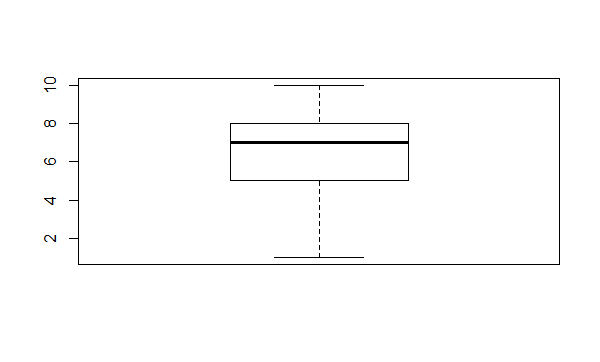
\includegraphics[width=0.7\linewidth]{Rplot2}
			\caption{Boxplot của AttractiveM}
			\label{fig:rplot2}
		\end{figure}
		
		Ta thấy rằng, dữ liệu này khá tốt khi không có ngoại lệ nhưng để chắc chắn thì ta sẽ kiểm định khoảng tin cậy cho trung vị của AttractiveM.
		
		\begin{lstlisting}[language=R]
		# Cac TK can tinh
		stat <- function(data){
			return (median(data)) # Median
		}
		
		# Bootstrap
		bootstrap <- function(B){
			return (replicate(B, stat(sample(data, length(data), replace = TRUE))))
		}
		
		# Lay du lieu
		data <- AttractiveM
		
		> (alpha <- 1 - 0.95)
		[1] 0.05
		> boots_dist <- bootstrap(10000) # Tim phan phoi cua bootstrap
		> (se <- sd(boots_dist, na.rm = TRUE)) # Tinh standard deviation (missing value se bi bo qua)
		[1] 0.3364154
		> (conf_boots <- quantile(boots_dist, c(alpha/2, 1 - alpha/2), na.rm = TRUE)) # Tim khoang tin cay cho median
		2.5% 97.5% 
		6     7
		\end{lstlisting}
		Vậy sai số chuẩn xấp xỉ bằng bootstrap là 0.3364154 và khoảng tin cậy 95\% cho $med$ dựa trên bootstrap
		là [6, 7].
	\end{enumerate}
	
	\textbf{Nhận xét:}
	\begin{itemize}
		\item Khoảng tin cậy chệch lệch giữa $med$ và $\mu$:
		$$[6, 7] - [6.491667, 6.896014] = [-0.491667, 0.103986]$$
		\item Ta thấy rằng chênh lệch này rất bé do đó dữ liệu không có outlier và phân bố dữ liệu có dạng bell shape đối xứng hai bên.
	\end{itemize}

	\subsubsection{LikeM (0-10)}
	\begin{enumerate}[label = \alph*)]
		\item Xây dựng khoảng tin cậy cho kì vọng
		
		Giả sử, ta cần khảo sát kì vọng (mean) mức độ thích của nam (0,1,...,10) đối với nữ cho quần thể (population) là toàn bộ sinh viên nam của trường Columbia. Từ tổng thể, ta thu thập được một mẫu dữ liệu ngẫu nhiên (random sample) gồm 276 quan sát. Dựa vào mẫu dữ liệu này, ta xây dựng khoảng tin cậy (confident interval) 95\% cho kì vọng mức độ thích của sinh viên nam trường.
	
	Gọi $\mu$ là mức độ thích trung bình của sinh viên nam trong trường, $\bar{x}$ là mức độ thích trung bình của sinh nam trong mẫu dữ liệu. Ta có
		$$\bar{x} = \frac{\sum_{i = 1}^{N}x_i}{N} =  6.682$$
	\begin{lstlisting}[language=R]
	# Cac TK can tinh
	stat <- function(data){
		return (mean(data)) # Mean
	}
	
	# Bootstrap
	bootstrap <- function(B){
		return (replicate(B, stat(sample(data, length(data), replace = TRUE))))
	}
	
	# Lay du lieu
	data <- LikeM
	
	> (alpha <- 1 - 0.95)
	[1] 0.05
	> boots_dist <- bootstrap(10000) # Tim phan phoi cua bootstrap
	> (se <- sd(boots_dist, na.rm = TRUE)) # Tinh standard deviation (missing value se bi bo qua)
	[1] 0.1064058
	> (conf_boots <- quantile(boots_dist, c(alpha/2, 1 - alpha/2), na.rm = TRUE)) # Tim khoang tin cay cho mean
	2.5%    97.5% 
	6.459013 6.877944
	\end{lstlisting}
	Vậy sai số chuẩn xấp xỉ bằng bootstrap là 0.1064058 và khoảng tin cậy 95\% cho $med$ dựa trên bootstrap
	là [6.459013, 6.877944].
		\item Xây dựng khoảng tin cây cho median
		
		Giả sử cùng tổng thể và mẫu dữ liệu ở câu a nhưng ta muốn xây dựng khoảng tin cậy 95\% cho
		trung vị (median) thay vì trung bình của mức độ thích. Mặc dù trung bình thường được sử dụng như
		là con số mô tả trọng tâm của phân phối nhưng nó lại rất nhạy cảm với ngoại lệ (outlier).
		
		Gọi $med$ là median mức độ thích của nam đối với nữ trong trường, $\hat{med}$ là median mức độ thích của nam đối với nữ trong mẫu dữ liệu. Ta có
		$$\hat{med} = 7.000$$
		
		Ta có thể thấy các ngoại lệ qua boxplot sau đây:
		\begin{figure}[H]
			\centering
			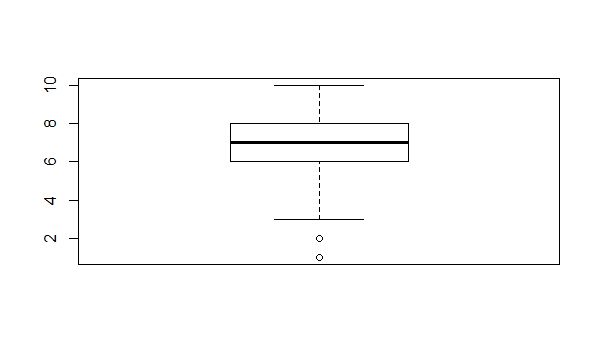
\includegraphics[width=0.7\linewidth]{Rplot1}
			\caption{Boxplot của LikeM}
			\label{fig:rplot1}
		\end{figure}
		
		Ta thấy rằng có một số outliers dưới 3 điểm. Trong những trường hợp như thế này ta có thể dùng trung vị là một thống kê ít bị ảnh hưởng bởi ngoại lệ.
		
		\begin{lstlisting}[language=R]
		# Cac TK can tinh
		stat <- function(data){
			return (median(data)) # Median
		}
		
		> (alpha <- 1 - 0.95)
		[1] 0.05
		> boots_dist <- bootstrap(10000) # Tim phan phoi cua bootstrap
		> (se <- sd(boots_dist, na.rm = TRUE)) # Tinh standard deviation (missing value se bi bo qua)
		[1] 0.06184588
		> (conf_boots <- quantile(boots_dist, c(alpha/2, 1 - alpha/2), na.rm = TRUE)) # Tim khoang tin cay cho median
		2.5% 97.5% 
		7     7 
		\end{lstlisting}
		Vậy sai số chuẩn xấp xỉ bằng bootstrap là 0.06184588 và khoảng tin cậy 95\% cho $med$ dựa trên bootstrap
		là [7, 7].
	\end{enumerate}
	\textbf{Nhận xét:}
	\begin{itemize}
		\item Khoảng tin cậy chênh lệch giữa $med$ và $\mu$:
			$$[7, 7] - [6.459013, 6.877944] = [0.122056, 0.540987]$$
		\item Ta thấy rằng, $med$ lớn hơn $\mu$ một chút. Suy ra, phân bố dữ liệu hơi bị lệch về bên trái.
	\end{itemize}
	\subsubsection{SincereM (0-10)}
	\begin{enumerate}[label = \alph*)]
	\item Xây dựng khoảng tin cậy cho kì vọng
	
	Giả sử, ta cần khảo sát kì vọng (mean) mức độ chân thành (0,1,...,10) của nữ cho quần thể (population) là toàn bộ sinh viên nữ của trường Columbia. Từ tổng thể, ta thu thập được một mẫu dữ liệu ngẫu nhiên (random sample) gồm 276 quan sát. Dựa vào mẫu dữ liệu này, ta xây dựng khoảng tin cậy (confident interval) 95\% cho kì vọng mức độ chân thành của sinh viên nữ trường.
	
	Gọi $\mu$ là mức độ chân thành trung bình của sinh viên nữ trong trường, $\bar{x}$ là mức độ thích chân thành của sinh nữ trong mẫu dữ liệu. Ta có
	$$\bar{x} = \frac{\sum_{i = 1}^{N}x_i}{N} =  7.856$$
	\begin{lstlisting}[language=R]
	# Cac TK can tinh
	stat <- function(data){
		return (mean(data)) # Mean
	}
	
	# Bootstrap
	bootstrap <- function(B){
		return (replicate(B, stat(sample(data, length(data), replace = TRUE))))
	}
	
	# Lay du lieu
	data <- SincereM
	
	> (alpha <- 1 - 0.95)
	[1] 0.05
	> boots_dist <- bootstrap(10000) # Tim phan phoi cua bootstrap
	> (se <- sd(boots_dist, na.rm = TRUE)) # Tinh standard deviation (missing value se bi bo qua)
	[1] 0.08472155
	> (conf_boots <- quantile(boots_dist, c(alpha/2, 1 - alpha/2), na.rm = TRUE)) # Tim khoang tin cay cho mean
	2.5%    97.5% 
	7.729710 8.008696 
	\end{lstlisting}
	Vậy sai số chuẩn xấp xỉ bằng bootstrap là 0.08472155 và khoảng tin cậy 95\% cho $med$ dựa trên bootstrap
	là [7.729710, 8.008696].
	\item Xây dựng khoảng tin cây cho median
	
	Giả sử cùng tổng thể và mẫu dữ liệu ở câu a nhưng ta muốn xây dựng khoảng tin cậy 95\% cho
	trung vị (median) thay vì trung bình của mức độ chân thành. Mặc dù trung bình thường được sử dụng như
	là con số mô tả trọng tâm của phân phối nhưng nó lại rất nhạy cảm với ngoại lệ (outlier).
	
	Gọi $med$ là median mức độ chân thành của nữ trong trường, $\hat{med}$ là median mức độ chân thành trong mẫu dữ liệu. Ta có
	$$\hat{med} = 8.000$$
	
	Ta có thể thấy các ngoại lệ qua boxplot sau đây:
	\begin{figure}[H]
		\centering
		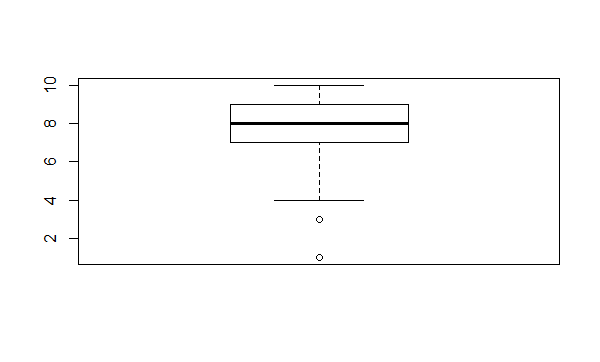
\includegraphics[width=0.7\linewidth]{Rplot3}
		\caption{Boxplot của LikeM}
		\label{fig:rplot1}
	\end{figure}
	
	Ta thấy rằng có một số outliers dưới 4 điểm. Trong những trường hợp như thế này ta có thể dùng trung vị là một thống kê ít bị ảnh hưởng bởi ngoại lệ.
	
	\begin{lstlisting}[language=R]
	# Cac TK can tinh
	stat <- function(data){
		return (median(data)) # Median
	}
	
	> (alpha <- 1 - 0.95)
	[1] 0.05
	> boots_dist <- bootstrap(10000) # Tim phan phoi cua bootstrap
	> (se <- sd(boots_dist, na.rm = TRUE)) # Tinh standard deviation (missing value se bi bo qua)
	[1] 0
	> (conf_boots <- quantile(boots_dist, c(alpha/2, 1 - alpha/2), na.rm = TRUE)) # Tim khoang tin cay cho median
	2.5% 97.5% 
	8     8
	\end{lstlisting}
	Vậy sai số chuẩn xấp xỉ bằng bootstrap là 0.0 và khoảng tin cậy 95\% cho $med$ dựa trên bootstrap
	là [8, 8].
	\end{enumerate}
	\textbf{Nhận xét:}
	\begin{itemize}
		\item Khoảng tin cậy chênh lệch giữa $med$ và $\mu$:
		$$[8, 8] - [7.729710, 8.008696] = [-0.008696, 0.270290]$$
		\item Ta thấy rằng, $med$ lớn hơn $\mu$. Suy ra, phân bố dữ liệu bị lệch về bên trái.
	\end{itemize}
	\section{Khảo sát cặp biến}
	\subsection{Biến định tính vs biến định tính}
	Chọn 2 biến định tính: DecisionMale (Yes/No) và RaceF (Asian, Black, Caucasian, Latino, Other)
	
	Khảo sát 2 biến định tính DecisionMale và RaceF
	
	\begin{lstlisting}[language=R]
	# 2 bien dinh tinh
	tab1 = table(DecisionMale, RaceF)
	# Them margin
	addmargins(tab1)
	>
	 RaceF
	DecisionMale     Asian Black Caucasian Latino Other Sum
	No    2    32     7        72      7    10 130
	Yes   2    38     8        76     16     6 146
	Sum   4    70    15       148     23    16 276
	
	# 2-way table
	# Ti le chung toc nu (Asian, Black, ...) nhan phan hoi
	prop.table(tab1, margin = 1)
	>
	            RaceF
	DecisionMale                 Asian      Black  Caucasian     Latino      Other
	No  0.01538462 0.24615385 0.05384615 0.55384615 0.05384615 0.07692308
	Yes 0.01369863 0.26027397 0.05479452 0.52054795 0.10958904 0.04109589
	
	barplot(tab1, legend = TRUE)
	\end{lstlisting}
	\begin{figure}[H]
		\centering
		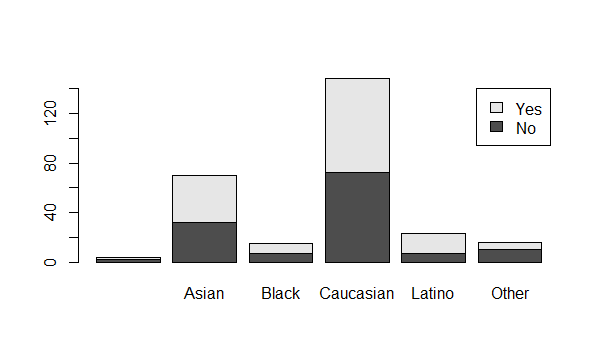
\includegraphics[width=0.7\linewidth]{Rplot4}
		\caption{Segmented barchart của DecisionMale và RaceF}
		\label{fig:rplot4}
	\end{figure}
	

	
	\subsubsection{Xây dựng khoảng tin cậy cho tỉ lệ khác biệt giữa nữ da trắng nhận phản hồi "Yes" và "No"}
		Giả sử, ta cần khảo sát tỉ lệ khác biệt giữa nữ da trắng được nam phản hồi (Yes/No) cho quần thể (population) là toàn bộ sinh viên nữ của trường Columbia bằng cách gom nhóm các dân tộc nữ khác còn lại thành 1 cụm.\\
		
		Ta chỉ phân tích giữa tỉ lệ nữ da trắng và nhóm khác. Từ tổng thể, ta thu thập được một mẫu dữ liệu ngẫu nhiên (random sample) gồm 276 quan sát trong đó có 148 nữ da trắng (gồm 76 phản hồi "Yes", 72 phản hồi "No") và 128 dân tộc khác (gồm 70 phản hồi "Yes" và 58 phản hồi "No").\\
		
		Dựa vào mẫu dữ liệu này, ta xây dựng khoảng tin cậy (confident interval) 95\% cho tỉ lệ khác biệt giữa nữ da trắng nhận phản hồi "Yes"/"No" của trường.\\
		
		Gọi $p_{Yes}$ là tỉ lệ nữ da trắng nhận phản hồi "Yes" và $p_{No}$ là tỉ lệ nữ da trắng nhận phản hồi "No". Từ đây, suy ra tỉ lệ khác biệt giữa $p_{Yes}$ và $p_{No}$ là $p_{Yes} - p_{No}$.
		
		\begin{lstlisting}[language=R]
		# Cac TK can tinh
		stat <- function(data){
			return (sum(data$DecisionMale == 'Yes' & data$RaceF == 'Caucasian')/ sum(data$DecisionMale == 'Yes') - sum(data$DecisionMale == 'No' & data$RaceF == 'Caucasian')/ sum(data$DecisionMale == 'No'))
		}
		
		# Bootstrap
		bootstrap <- function(B){
			return (replicate(B, stat(sample(data, nrow(data), replace = TRUE))))
		}
		
		# Concatenate 2 column
		data <- data.frame(DecisionMale, RaceF)
		
		> (alpha <- 1 - 0.95)
		[1] 0.05
		> boots_dist <- bootstrap(10000) # Tim phan phoi cua bootstrap
		> (se <- sd(boots_dist, na.rm = TRUE)) # Tinh standard deviation (missing value se bi bo qua)
		[1] 0.05991396
		> (conf_boots <- quantile(boots_dist, c(alpha/2, 1 - alpha/2), na.rm = TRUE)) # Tim khoang tin cay cho p
		2.5%       97.5% 
		-0.15182990  0.08478168 
		\end{lstlisting}
		Vậy sai số chuẩn xấp xỉ bằng bootstrap là 0.05991396 và khoảng tin cậy 95\% cho $p_{Yes} - p_{No}$ dựa trên bootstrap là [-0.15182990, 0.08478168].\\
		
		\textbf{Nhận xét:}
		\begin{itemize}
			\item Ta thấy rằng khoảng tin cậy cho tỉ lệ khác biệt $p_{Yes} - p_{No}$ là [-0.15182990, 0.08478168]. Ta có thể kết luận rằng, $p_{Yes} \leq p_{No}$.
			\item Điều này cho thấy nữ da trắng nhận được phản hồi "Yes" ít hơn hoặc bằng "No".
		\end{itemize}
		
		\subsubsection{Xây dựng khoản tin cậy cho tỉ lệ khác biệt giữa nữ châu Á nhận phản hồi "Yes"/"No"}
		
			Giả sử, ta cần khảo sát tỉ lệ khác biệt giữa nữ châu Á được nam phản hồi (Yes/No) cho quần thể (population) là toàn bộ sinh viên nữ của trường Columbia bằng cách gom nhóm các dân tộc nữ khác còn lại thành 1 cụm.\\
			
			Ta chỉ phân tích giữa tỉ lệ nữ châu Á và nhóm khác. Từ tổng thể, ta thu thập được một mẫu dữ liệu ngẫu nhiên (random sample) gồm 276 quan sát trong đó có 70 nữ châu Á (gồm 32 phản hồi "Yes", 32 phản hồi "No") và 206 dân tộc khác (gồm 108 phản hồi "Yes" và 98 phản hồi "No").\\
			
			Dựa vào mẫu dữ liệu này, ta xây dựng khoảng tin cậy (confident interval) 95\% cho tỉ lệ khác biệt giữa nữ châu Á nhận phản hồi "Yes"/"No" của trường.\\
		
		Gọi $p_{Yes}$ là tỉ lệ nữ châu Á nhận phản hồi "Yes" và $p_{No}$ là tỉ lệ nữ châu Á nhận phản hồi "No". Từ đây, suy ra tỉ lệ khác biệt giữa $p_{Yes}$ và $p_{No}$ là $p_{Yes} - p_{No}$.
		
		\begin{lstlisting}[language=R]
		# Cac TK can tinh
		stat <- function(data){
			return (sum(data$DecisionMale == 'Yes' & data$RaceF == 'Asian')/sum(data$DecisionMale == 'Yes') - sum(data$DecisionMale == 'No' & data$RaceF == 'Asian')/ sum(data$DecisionMale == 'No'))
		}
		
		> (alpha <- 1 - 0.95)
		[1] 0.05
		> boots_dist <- bootstrap(10000) # Tim phan phoi cua bootstrap
		> (se <- sd(boots_dist, na.rm = TRUE)) # Tinh standard deviation (missing value se bi bo qua)
		[1] 0.05236749
		> (conf_boots <- quantile(boots_dist, c(alpha/2, 1 - alpha/2), na.rm = TRUE)) # Tim khoang tin cay cho p
		2.5%       97.5% 
		-0.08825722  0.11742327
		\end{lstlisting}
		Vậy sai số chuẩn xấp xỉ bằng bootstrap là 0.05236749 và khoảng tin cậy 95\% cho $p_{Yes} - p_{No}$ dựa trên bootstrap là [-0.08825722, 0.11742327].\\
		
		\textbf{Nhận xét:}
		\begin{itemize}
			\item Ta thấy rằng khoảng tin cậy cho tỉ lệ khác biệt $p_{Yes} - p_{No}$ là [-0.08825722, 0.11742327]. Ta có thể kết luận rằng, $p_{Yes} \sim p_{No}$.
			\item Điều này cho thấy nữ da trắng nhận được phản hồi "Yes" tương đối bằng "No".
		\end{itemize}
	\subsection{Biến định tính và biến định lượng}
	Chon 1 biến định tính và 1 biến định lượng: ̣DecisionMale (yes/no), AttractiveM (1-10)
	\begin{lstlisting}[language = R]
	# Tinh favorite statistics
	> favstats(AttractiveM ~ DecisionMale)
	DecisionMale min Q1 median Q3 max     mean       sd   n missing
	1           No   1  5      5  6  10 5.641732 1.694877 127       3
	2          Yes   5  7      8  8  10 7.595890 1.357375 146       0
	
	# Ve boxplot
	boxplot(AttractiveM ~ DecisionMale, xlab = "DecisionMale", ylab = "AttractiveM")
	\end{lstlisting}
	\begin{figure}[H]
		\centering
		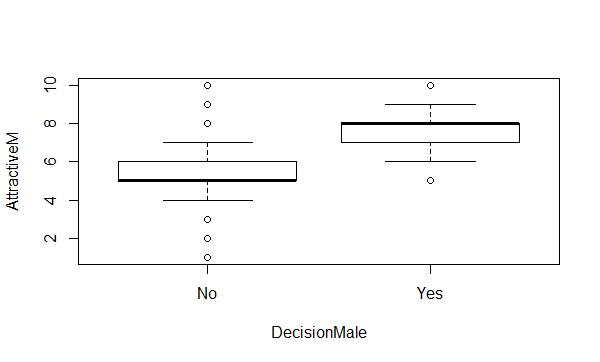
\includegraphics[width=0.7\linewidth]{Rplot5}
		\caption{Side-by-side boxplots}
		\label{fig:rplot5}
	\end{figure}
	
	\subsubsection{Xây dựng khoảng tin cậy cho độ chênh lệch kì vọng giữa mức độ hấp dẫn của nữ trong phản hồi "Yes" và mức độ hấp dẫn của nữ trong phản hồi "No"}
	
	Giả sử, ta cần khảo sát kì vọng chênh lệch giữa mức độ hấp dẫn của nữ trong phản hồi "Yes" và trong phản hồi "No" cho quần thể (population) là toàn bộ sinh viên nữ của trường Columbia.\\
	
	Từ tổng thể, ta thu thập được một mẫu dữ liệu ngẫu nhiên (random sample) gồm 276 quan sát. Dựa vào mẫu dữ liệu này, ta xây dựng khoảng tin cậy (confident interval) 95\% cho sự chênh lệch kì vọng giữa mức độ hấp dẫn của nữ nhận phản hồi "Yes"/"No" của trường.\\
	
	Gọi $\mu_{AttractiveM|Yes}$ là kì vọng mức độ hấp dẫn của nữ nhận phản hồi "Yes" và $\mu_{AttractiveM|No}$ là kì vọng mức độ hấp dẫn của nữa nhận phản hồi "No" trong trường.\\
	
	$\bar{x}_{AttractiveM|Yes}$ là mức độ hấp dẫn trung bình của nữ nhận phản hồi "Yes" và $\bar{x}_{AttractiveM|No}$ là mức độ hấp dẫn trung bình của nữ nhận phản hồi "No" trong mẫu dữ liệu. Từ các thống kê tính được bằng R, ta có:
	$$\bar{x}_{AttractiveM|Yes} = 7.595890, \bar{x}_{AttractiveM|No} = 5.641732$$
	
	Từ đây, suy ra độ chênh lệch kì vọng giữa $\mu_{AttractiveM|Yes}$ và $\mu_{AttractiveM|No}$ là $\mu_{AttractiveM|Yes} - \mu_{AttractiveM|No}$.
	
	\begin{lstlisting}[language=R]
	# Cac TK can tinh
	stat <- function(data){
		#Tinh mean cho no va yes
		mean2 <- mean(data$AttractiveM~data$DecisionMale, na.rm = TRUE)
		return (mean2[2] - mean2[1])
	}
	
	# Bootstrap
	bootstrap <- function(B){
		return (replicate(B, stat(sample(data, nrow(data), replace = TRUE))))
	}
	
	# Concatenate 2 column
	data <- data.frame(DecisionMale, AttractiveM)
	
	> (alpha <- 1 - 0.95)
	[1] 0.05
	> boots_dist <- bootstrap(10000) # Tim phan phoi cua bootstrap
	> (se <- sd(boots_dist, na.rm = TRUE)) # Tinh standard deviation (missing value se bi bo qua)
	[1] 0.1874891
	> (conf_boots <- quantile(boots_dist, c(alpha/2, 1 - alpha/2), na.rm = TRUE)) # Tim khoang tin cay cho mean
	2.5%    97.5% 
	1.582028 2.317613
	\end{lstlisting}
	Vậy sai số chuẩn xấp xỉ bằng bootstrap là 0.1874891 và khoảng tin cậy 95\% cho $\mu_{AttractiveM|Yes} - \mu_{AttractiveM|No}$ dựa trên bootstrap là [1.582028, 2.317613].\\
	
	\textbf{Nhận xét:}
	\begin{itemize}
		\item Ta thấy rằng khoảng tin cậy cho tỉ lệ khác biệt $\mu_{AttractiveM|Yes} - \mu_{AttractiveM|No}$ là [1.582028, 2.317613]. Ta có thể kết luận rằng, $\mu_{AttractiveM|Yes} > \mu_{AttractiveM|No} $.
		\item Điều này cho thấy kì vọng mức độ hấp dẫn nữ da trắng nhận được phản hồi "Yes" cao hơn "No". Điều này cũng khá hiển nhiên theo cách suy nghĩ trực quan của chúng ta.
	\end{itemize}

	\subsubsection{Xây dựng khoảng tin cậy cho độ chênh lệch trung vị giữa mức độ hấp dẫn của nữ trong phản hồi "Yes" và mức độ hấp dẫn của nữ trong phản hồi "No"}
	
	Giả sử cùng tổng thể và mẫu dữ liệu ở câu trên nhưng ta muốn xây dựng khoảng tin cậy 95\% cho
	trung vị (median) thay vì trung bình của mức độ hấp dẫn trong phản hồi "Yes"/"No". Mặc dù trung bình thường được sử dụng như là con số mô tả trọng tâm của phân phối nhưng nó lại rất nhạy cảm với ngoại lệ (outlier).\\
	
	Ta có thể thấy trong \ref{fig:rplot5} ở mỗi phản hồi "Yes" và "No" đều có các outlier xuất hiện đặc biết nhất là ở phản hồi "No", có những điểm số bất thường như 8, 9, 10 vẫn nằm trong phản hồi "No".\\
	
	Gọi $med_{AttractiveM|Yes}$ là median mức độ hấp của nữ trong phản hồi "Yes" và $med_{AttractiveM|No}$ là median mức độ hấp của nữ trong phản hồi "No" của trường.\\
	
	Gọi $\hat{med}_{AttractiveM|Yes}$ là median mức độ hấp dẫn của nữ trong phản hồi "Yes" và  $\hat{med}_{AttractiveM|No}$ là median mức độ hấp dẫn của nữ trong phản hồi "No" của mẫu dữ liệu. Từ các thống kê tính được bằng R, ta có:
	$$\hat{med}_{AttractiveM|Yes} = 8, \hat{med}_{AttractiveM|No} = 5$$
	
	Ta có thể thấy rằng, median kháng nhiễu tốt hơn so với mean dựa vào số liệu thống kê trên.\\
	
	\begin{lstlisting}[language=R]
	# Cac TK can tinh
	stat <- function(data){
		#Tinh median cho no va yes
		med2 <- median(data$AttractiveM~data$DecisionMale, na.rm = TRUE)
		return (med2[2] - med2[1])
	}
	
	> (alpha <- 1 - 0.95)
	[1] 0.05
	> boots_dist <- bootstrap(10000) # Tim phan phoi cua bootstrap
	> (se <- sd(boots_dist, na.rm = TRUE)) # Tinh standard deviation (missing value se bi bo qua)
	[1] 0.5664177
	> (conf_boots <- quantile(boots_dist, c(alpha/2, 1 - alpha/2), na.rm = TRUE)) # Tim khoang tin cay cho median
	2.5% 97.5% 
	1     3 
	\end{lstlisting}
	Vậy sai số chuẩn xấp xỉ bằng bootstrap là 0.5664177 và khoảng tin cậy 95\% cho $med_{AttractiveM|Yes} - med_{AttractiveM|No}$ dựa trên bootstrap là [1, 3].\\
	
	\textbf{Nhận xét:}
	\begin{itemize}
		\item Ta có $se = 0.5664177$ sai số này khá cao.
		\item Ta thấy rằng khoảng tin cậy cho tỉ lệ khác biệt $med_{AttractiveM|Yes} - med_{AttractiveM|No}$ là [1, 3]. Ta có thể kết luận rằng, $med_{AttractiveM|Yes} > med_{AttractiveM|No} $.
		\item Ta thấy rằng với khoảng tin cậy cho median thì kháng nhiễu và phản ánh đúng hơn so với mean.
		\item Điều này cho thấy trụng vị mức độ hấp dẫn nữ da trắng nhận được phản hồi "Yes" cao hơn "No". Điều này cũng khá hiển nhiên theo cách suy nghĩ trực quan của chúng ta.
	\end{itemize}
	
	\subsection{Biến định lượng và biến định lượng}
	Chọn 2 biến định lượng: AttractiveM (1-10) và LikeM (1-10)
	\begin{lstlisting}[language=R]
	# Correlation of 2 quantative variables: AttractiveM and LikeM
	> cor(AttractiveM, LikeM, use = "complete.obs") # Avoid missing values
	[1] 0.7240187
	
	# Fit regression line
	lmInfo <- lm(LikeM~AttractiveM)
	> summary(lmInfo) # get more info
	Call:
	lm(formula = LikeM ~ AttractiveM)
	
	Residuals:
	Min      1Q  Median      3Q     Max 
	-4.6225 -0.6225  0.0914  0.8054  3.6611 
	
	Coefficients:
	Estimate Std. Error t value Pr(>|t|)    
	(Intercept)  1.91100    0.28616   6.678 1.37e-10 ***
	AttractiveM  0.71394    0.04132  17.279  < 2e-16 ***
	---
	Signif. codes:  0 ‘***’ 0.001 ‘**’ 0.01 ‘*’ 0.05 ‘.’ 0.1 ‘ ’ 1
	
	Residual standard error: 1.232 on 271 degrees of freedom
	(3 observations deleted due to missingness)
	Multiple R-squared:  0.5242,	Adjusted R-squared:  0.5224 
	F-statistic: 298.6 on 1 and 271 DF,  p-value: < 2.2e-16
	
	# Graphical display: scatterplot
	plot(AttractiveM, LikeM, main = "Scatter plot example", pch=19)
	# Add fit lines
	abline(lm(LikeM~AttractiveM), col="red") # regression line (y~x)
	
	plot(lmInfo$residuals, pch = 16, col = "red") #Plot residual de xem du lieu co phan bo ngau nhieu khong?
	\end{lstlisting}
	
	\begin{figure}[H]
		\centering
		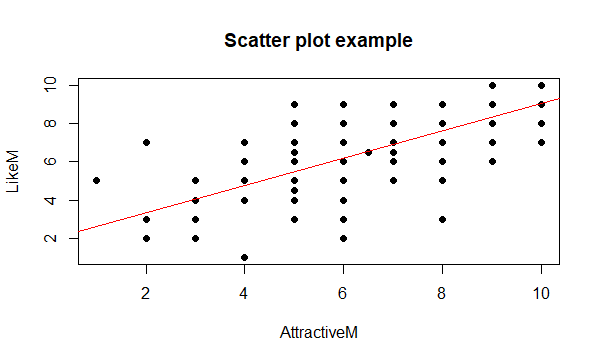
\includegraphics[width=0.7\linewidth]{Rplot6}
		\caption{Scatterplot của 2 biến định lượng và có linear regression line}
		\label{fig:rplot6}
	\end{figure}
	
	\begin{figure}[H]
		\centering
		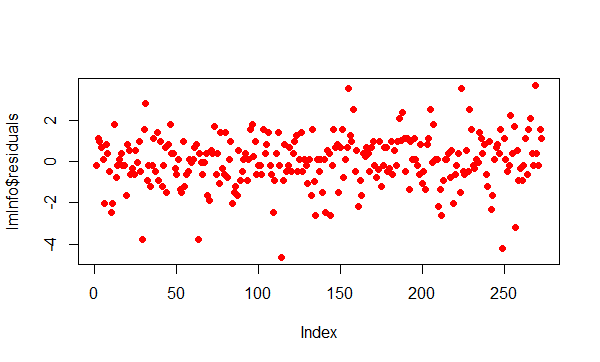
\includegraphics[width=0.7\linewidth]{Rplot7}
		\caption{Residuals plot}
		\label{fig:rplot7}
	\end{figure}
	
	\textbf{Nhận xét:}
	\begin{itemize}
		\item Nhìn vào Residuals, ta thấy rằng độ lệch giữa giá trị dự đoán và giá trị quan sát vẫn còn chệnh lệch khá nhiều.
		\item Tiếp theo, để đánh giá model này có tốt hay không thì ta cần nhìn vào $R^2 = 0.5242$ thì ta thấy nó gần 0.5. Điều này có thể tạm chấp nhận là model này khá tốt.
		\item Nhưng đến đây ta chưa thể vội kết luận rằng model này tốt. Do đó, ta cần plot residuals để xem phân bố của chúng có ngẫu nhiên không. Nếu không ngẫu nhiên mà có thể là có 1 hidden pattern mà model chưa xét tới. Điều này sẽ ảnh hưởng đến khả năng dự đoán khi mà dữ liệu tăng.
		\item Nhìn vào hình \ref{fig:rplot7}, ta đã có thể yên tâm kết luận rằng model này là tốt vì các residuals phân bố ngẫu nhiên (không có hidden pattern như: curve,...)
	\end{itemize}
	
	\subsubsection{Xây dựng khoảng tin cậy cho hệ số tương quan giữa AttractiveM và LikeM}
	Giả sử, ta cần khảo sát hệ số tương quan (correlation coefficient) giữa mức độ hấp dẫn và mức độ thích của nam giới đánh giá cho nữ (AttractiveM và LikeM) cho quần thể (population) là toàn bộ sinh viên nữ của trường Columbia.\\
	
	Từ tổng thể, ta thu thập được một mẫu dữ liệu ngẫu nhiên (random sample) gồm 276 quan sát. Dựa vào mẫu dữ liệu này, ta xây dựng khoảng tin cậy (confident interval) 95\% cho hệ số tương quan giữa AttractiveM và LikeM.\\
	
	Gọi $\sigma$ là hệ số tương quan giữa AttractiveM và LikeM của sinh viên nữ trong trường và $s$ là hệ số tương quan giữa AttractiveM và LikeM của sinh viên nữ trong mẫu dữ liệu. Từ các thống kê tính được bằng R, ta có: $s = 0.7240187$
	
	\begin{lstlisting}[language=R]
	# Cac TK can tinh
	stat <- function(data){
	#Tinh correlation
		return (cor(data$AttractiveM, data$LikeM, use = "complete.obs")) # Avoid missing values
	
	}
	
	# Bootstrap
	bootstrap <- function(B){
		return (replicate(B, stat(sample(data, nrow(data), replace = TRUE))))
	}
	
	# Concatenate 2 column
	data <- data.frame(AttractiveM, LikeM)
	
	> (alpha <- 1 - 0.95)
	[1] 0.05
	> boots_dist <- bootstrap(10000) # Tim phan phoi cua bootstrap
	> (se <- sd(boots_dist, na.rm = TRUE)) # Tinh standard deviation (missing value se bi bo qua)
	[1] 0.03407269
	> (conf_boots <- quantile(boots_dist, c(alpha/2, 1 - alpha/2), na.rm = TRUE)) # Tim khoang tin cay cho correlation
	2.5%     97.5% 
	0.6528767 0.7859563
	\end{lstlisting}
		Vậy sai số chuẩn xấp xỉ bằng bootstrap là 0.03407269 và khoảng tin cậy 95\% cho $\sigma$ dựa trên bootstrap là [0.6528767, 0.7859563].\\
		
	\textbf{Nhận xét:}
	\begin{itemize}
		\item Ta có khoảng tin cậy cho $\sigma$ là [0.6528767, 0.7859563] có thể thấy rằng đây là 1 liên kết dương mạnh. 
		\item Điều này có nghĩa là mức độ hấp dẫn của nữ AttractiveM tăng thì mức độ thích của nam dành cho nữ LikeM cũng tăng.
	\end{itemize}
	
	\subsubsection{Xây dựng khoảng tin cậy cho hệ số a (intercept) và hệ số b (slope) của regression line}
	
	Giả sử, ta cần khảo sát best-fit line với 2 hệ số tương quan: a (intercept), b (slope) giữa mức độ hấp dẫn và mức độ thích của nam giới đánh giá cho nữ (AttractiveM và LikeM) cho quần thể (population) là toàn bộ sinh viên nữ của trường Columbia.\\
	
	Từ tổng thể, ta thu thập được một mẫu dữ liệu ngẫu nhiên (random sample) gồm 276 quan sát. Dựa vào mẫu dữ liệu này, ta xây dựng khoảng tin cậy (confident interval) 95\% cho hệ số tương quan a, b giữa AttractiveM và LikeM.\\
	
	Gọi $a, b$ lần lượt hệ số intercept và slope của regression line giữa AttractiveM và LikeM của sinh viên nữ trong trường và $\hat{a}, \hat{b}$ lần lượt hệ số intercept và slope của regression line giữa AttractiveM và LikeM của sinh viên nữ trong mẫu dữ liệu. Từ các thống kê tính được bằng R, ta có: 
	$$\hat{a} =  1.91100, \hat{b} = 0.71394$$
	
	\begin{lstlisting}[language=R]
	# Cac TK can tinh
	stat <- function(data){
	#Tim best-fit line
	lmInfo <- lm(data$LikeM~data$AttractiveM)
	return (lmInfo$coefficients) # Avoid missing values
	}
	
	# Bootstrap
	bootstrap <- function(B){
	return (replicate(B, stat(sample(data, nrow(data), replace = TRUE))))
	}
	
	# Concatenate 2 column
	data <- data.frame(AttractiveM, LikeM)
	
	(alpha <- 1 - 0.95)
	boots_dist <- bootstrap(10000) # Tim phan phoi cua bootstrap
	
	# Tim sai lech chuan va khoang tin cay cho he so a
	> a_dist <- boots_dist[seq(1, 10000, by = 2)]
	> (se <- sd(a_dist, na.rm = TRUE)) # Tinh standard deviation (missing value se bi bo qua)
	[1] 0.3547863
	> (conf_boots <- quantile(a_dist, c(alpha/2, 1 - alpha/2), na.rm = TRUE)) # Tim khoang tin cay cho a
	2.5%    97.5% 
	1.210695 2.600174 
	
	# Tim sai lech chuan va khoang tin cay cho he so b
	> b_dist <- boots_dist[seq(2, 10000, by = 2)]
	> (se <- sd(b_dist, na.rm = TRUE)) # Tinh standard deviation (missing value se bi bo qua)
	[1] 0.04883863
	> (conf_boots <- quantile(b_dist, c(alpha/2, 1 - alpha/2), na.rm = TRUE)) # Tim khoang tin cay cho b
	2.5%     97.5% 
	0.6184535 0.8112570
	\end{lstlisting}
	Vậy sai số chuẩn xấp xỉ bằng bootstrap cho hệ số $a$ là 0.3547863 và khoảng tin cậy 95\% cho $a$ dựa trên bootstrap là [1.210695, 2.600174] và sai số chuẩn xấp xỉ bằng bootstrap cho hệ số $b$ là 0.04883863 và khoảng tin cậy 95\% cho $b$ dựa trên bootstrap là [0.6184535, 0.8112570].
	
	\section{Tham khảo}
		\label{Tham khao}
		\begin{enumerate}[label=$\lbrack$\arabic*$\rbrack$]
			\item Randall Pruim and Lana Park. Lock5WithR. Chapter 3: Confident interval. PDF. 
			\item R Users Guide. Chapter 3: Confident interval. PDF.
			\item "Linear Regression R." DataCamp Community. \url{https://www.datacamp.com/community/tutorials/linear-regression-R}.
			\item Hoang, Vu Quoc and An, Le Huong Thao. LAB 05 – KHOẢNG TIN CẬY. PDF.
		\end{enumerate}
		 
	
\end{document}